\documentclass[a4paper]{article}

%% Language and font encodings
\usepackage[utf8]{inputenc}
\usepackage[ngerman]{babel}
\usepackage[T1]{fontenc}
\usepackage{caption}

%% Sets page size and margins
\usepackage[a4paper,top=3cm,bottom=2cm,left=3cm,right=3cm,marginparwidth=1.75cm]{geometry}

%% Useful packages
\usepackage{amsmath}
\usepackage{graphicx}
\usepackage[style=nature]{biblatex}
\usepackage[colorinlistoftodos]{todonotes}
\usepackage[colorlinks=true, allcolors=blue]{hyperref}
\usepackage{float}

\addbibresource{references.bib}

\title{Praktikum Neurobiologie - Protokoll 2}

\author{Cedric Laier, Tilman Mehl}


\begin{document}
%Titelpage Modell: https://www.latextemplates.com/template/formal-book-title-page
\begin{titlepage} % Suppresses headers and footers on the title page

	\centering % Centre everything on the title page
	
	\scshape % Use small caps for all text on the title page
	
	\vspace*{\baselineskip} % White space at the top of the page
	
	%------------------------------------------------
	%	Title
	%------------------------------------------------
	
	\rule{\textwidth}{1.6pt}\vspace*{-\baselineskip}\vspace*{2pt} % Thick horizontal rule
	\rule{\textwidth}{0.4pt} % Thin horizontal rule
%	{\LARGE THE BIG BOOK\\ OF\\ \LaTeX ~TEMPLATES\\} % Title
	\vspace{0.75\baselineskip} % Whitespace above the title
	{\LARGE Erregungsleitung im Bauchmark des Regenwurms} {\\Protokoll zum Praktikum Neurobiologie für Bioinformatiker\\ am 15.01.2019} % Title

	
	\vspace{0.75\baselineskip} % Whitespace below the title
	
	\rule{\textwidth}{0.4pt}\vspace*{-\baselineskip}\vspace{3.2pt} % Thin horizontal rule
	\rule{\textwidth}{1.6pt} % Thick horizontal rule
	
	\vspace{2\baselineskip} % Whitespace after the title block
	
	\vspace{2.0\baselineskip} % Whitespace before the editors

{\LARGE Gruppe 2}
\vspace{2.5\baselineskip} \\
	
{\LARGE Autoren:}
\begin{itemize}
\item Cedric Laier - \textit{cedric.laier@fu-berlin.de}
\item Tilman Mehl - \textit{tilmanmehl@zedat.fu-berlin.de}
\end{itemize}
\vspace{2.5\baselineskip}

{\LARGE Lehrveranstalter:}
\begin{itemize}
\item  Peter Robin Hiesinger
\item Matthias Wernet
\end{itemize}
\vspace{2.5\baselineskip}

{\LARGE Tutoren:}
\begin{itemize}
\item Lisa
\item Johannes
\item Claudia
\end{itemize}
	
\end{titlepage}
\section{Einleitung}

Inhalt des Praktikumstages war die Reizerzeugung und -weiterleitung an Neuronen.\\
Eine schnellere Erregungsleitung ermöglicht Organismen eine schnellere Reaktion auf Reize und damit eine Erhöhung der (evolutionären) Fitness. Uns sind zwei Lösungen bekannt, durch die die Reizweiterleitung beschleunigt werden kann.
\subsection{Myelinisierung von Axonen}
Eine Lösung, wie sie auch beim Menschen auftritt, ist die Myelinisierung.
Lipidreiche Gliazellen umwickeln die Neuronen und wirken so als Isolator. Dadurch wird effektiv der Membranwiderstand \(R_m\) erhöht und Leckströme vermindert.\\
\subsection{Ausbildung von Riesenaxonen}
Eine weitere Lösung, wie sie unter anderem beim Regenwurm auftritt, ist die Ausbildung von Riesenaxonen mit hohem Durchmesser.\\
Betrachtet man die Formel für den Längswiderstand \[R_i = \frac{R_m}{(\pi \cdot d)^2}\] erkennt man, dass dieser durch die Erhöhung des Durchmessers d geringer wird. Eine Verringerung des Längswiderstandes führt zu einer Erhöhung der Reizweiterleitung.

\section{Versuchsaufbau und -durchführung}
Im Rahmen des 2. Praktikumtages wurden verschiedene Experimente durchgeführt. Bei dem Versuchstier handelte es sich um einen Regenwurm (\textit{Lumbricus terrestris)}. Abhängig vom Experiment war jeweils ein unterschiedlicher Versuchsaufbau notwendig. Die nachfolgenden Unterkapitel sollen nun einen detaillierteren Einblick in Aufbau und Durchführung der Experimente geben.
\subsection{Versuchsaufbau}
Der Grundaufbau für unsere Messungen ist in Abbildung 1 zu sehen. Hier wurde eine von zwei Seiten, der in der Wurmplatte befindlichen Elektrodenpaare, mit dem Differenzverstärker verbunden. Der Differenzverstärker ist ein elektronischer Verstärker mit zwei Eingängen, bei dem die Differenz der beiden Eingangssignale verstärkt wird und das Herausfiltern von Fremdsignalen ermöglicht. Der Differenzverstärker wiederrum wurde mit einem Analog-Digital-Wandler verbunden, wodurch es uns möglich wurde die Signale digitalisiert mithilfe des Computers und dem sich darauf befindlichen Spike2 aufzuzeichnen und zu analysieren. \\ \\ 
In Abbildung 2 ist der erweiterte Versuchsaufbau zu sehen. Die Experimente zur Reizschwellen- und Fortleitungsgeschwindigkeitsmessung und bei der Bestimmung der Refraktärphase erforderten es das Versuchstier mithilfe eines Reizgenerators zu stimmulieren. Der Reizgenerator wurde hier mit dem zweiten Elektrodenpaar auf der Anteriorseite der Wurmplatte verbunden. Am Signal Ausgang des Reizgenerators wurde zusätzlich noch ein weiteres Kabelpaar montiert, welches mit einem Eingangsport des Analog-Digital-Wandlers verbunden wurde. Dadurch waren wir in der Lage dass gefeuerte Reizsignal des Reizgenerators mithilfe von Spike2 auch messen und aufzeichnen zu können.
\subsection{Versuchskizzen} 
\vspace{2.5\baselineskip}
\begin{figure}[H]
    \centering
    \captionsetup{justification=centering,margin=2cm}
    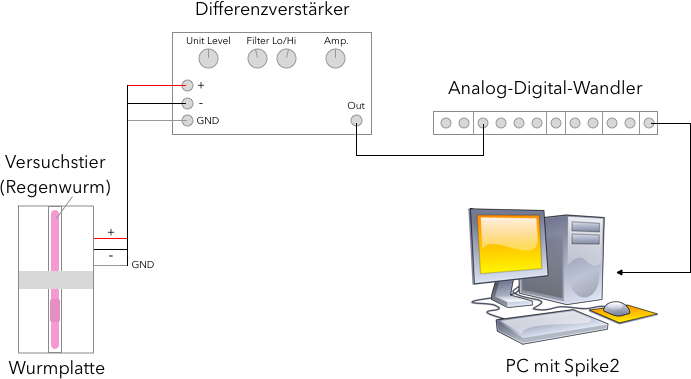
\includegraphics[scale=0.6]{images/Versuchsaufbau_Wurm.png}
    \caption{Skizze des Versuchsgrundaufbau}
\end{figure}

\vspace{2.5\baselineskip}
\begin{figure}[H]
    \centering
    \captionsetup{justification=centering,margin=2cm}
    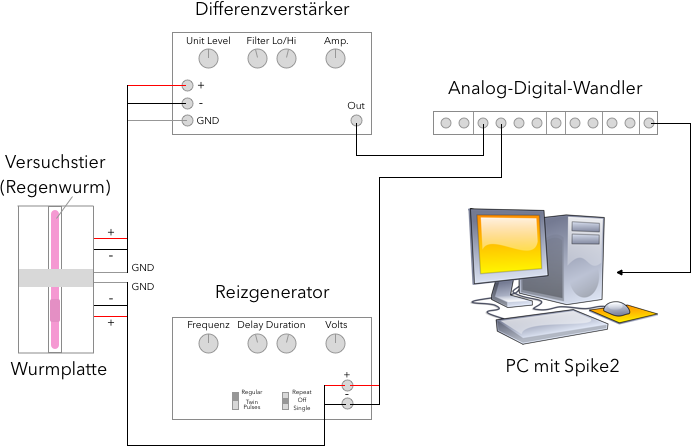
\includegraphics[scale=0.6]{images/Versuchsaufbau_Wurm_Reizgenerator.png}
    \caption{Skizze des Versuchsaufbau mit zusätzlich angeschlossenem Reizgenerator}
\end{figure}
\subsection{Versuchsdurchführung}
In diesem Kapitel thematisieren wir die Versuchsdurchführung der vier ausgeführten Experimente. Jedes Unterkapitel adressiert den Versuchsaufbau und die Durchführung der Experimente in ausführlicher Form, begleitend zu den Skizzen aus Kabitel 2.2.
\subsubsection{Lokomotion des Regenwurms}
Hier wurde der Regenwurm auf ein angefeuchtes Papier gelegt und seine Bewegungen beobachtet. Durch Berührungen der posterioren und anterioren Enden mithife eines stumpfen Holzspieß wurden seine Meidereaktionen von uns untersucht und protokolliert. 
\subsubsection{Identifikation der Riesenfaser bei mechanischer Reizung}
In Abbildung 1 ist der Versuchsaufbau skizziert mit welchem wir versucht haben die laterale und mediane Riesenfaser zu identifizieren. Hierzu haben wir den Wurm in die Wurmplatte kriechen lassen. Die Wurmplatte besitzt auf beiden Seiten zwei Elektrodenpaare über die der Wurm drüber kriecht, sodass eine Messung auf der Bauchseite möglich ist. Durch Knete wurde der sich im Wurmkanal befindene Wurm auf beiden Seiten blockiert, sodass er sich im Kanal nicht mehr bewegen konnte. Durch das Auflegen einer (mit kleinen Löchern versehenen) Plexiglas-Platte wurde auch der Weg nach oben blockiert. Wir begannen mit der Spike2 Aufzeichnung und der Wurm wurde anschließend von uns jeweils 5 mal auf anteriorer und posteriorer Seite durch die Löcher im Plexiglas mit einem stumpfen Holzspieß stimmuliert. Zwischen jeder Stimmulation wurden dem Wurm 30 Sekunden zur Erholung gegeben.
\subsubsection{Reizschwellen- und Fortleitungsgeschwindigkeitsmessung}
Für das dritte Experiment haben wir den Versuchsaufbau um einen Reizgenerator erweitert (siehe Abbildung 2). Hier wurde der Reizgenerator mit der anterioren Seite des Wurms (bzw. der Wurmplatte) verbunden. Die Reizdauer (Duration) wurde von uns auf 0,1 ms gesetzt und die Reizstärke (Volts) auf anfänglich 0,5 V. Nach einer doppelten Sichtung unsere Einstellungen starteten wir unsere Aufzeichnung. Nun feuerten wir einen Single-Puls ab und beobachteten unsere Messung. Wir wiederholten diesen Schritt alles 30 Sekunden und erhöhten bei jedem Single-Puls die Reizstärke in 0,5 V Schritten. Ziel war es den Zeitpunkt protokollieren zu können, bei dem zum ersten Mal ein Aktionspotential in den Aufzeichnungen sichtbar wurde.
\subsubsection{Bestimmung der Refraktärphasen bei elektrischer Reizung}
Im letzten Experiment war es das Ziel den zeitlichen Abstand zu finden bei dem auf zwei direkt aufeinander folgenden Reizen, nur noch ein Aktionspotential ausgelöst wird. Hierfür wurde der Impulstyp des Reizgenerators über einen Schiebeschalter von Single-Puls auf Twin-Puls gestellt und über den den Delay Knopf ein zeitlicher Abstand beider Impulse von 20ms festgelegt. Die Impulsstärke (Volts) wurde auf 4.0 Volt gestellt, weil dieser Wert (laut unseren Messungen) zur sicheren Erzeugung eines Aktionspotentials führte. Wir reduzierten nun wieder in 2 ms Schritten den Delay zwischen jedem abgefeuertem Twin-Puls und gaben dem Wurm anschließend immer mind. 30 Sekunden Erholungszeit. Dieses wiederholten wir bis wir einen Delay Wert erreicht hatten, bei dem nur noch ein Aktionspotential zu messen war. Anschließend haben wir mit diesem Delay Wert systematisch die Impulsstärke wieder erhöht bis erneut zwei Aktionspotentiale sichtbar wurden. Die Werte der Geräte und Messungen wurden anschließend notiert und von uns bestmöglich ausgewertet.

\newpage
\section{Ergebnisse}

\subsection{Lokomotion des Regenwurms}
Der Wurm führt mit dem anterioren Ende Tast- oder Suchbewegungen aus. \\
Zur Bewegung werden Segmente in die gewünschte Richtung gestreckt, verankert und kontrahiert, wodurch nachfolgende Segmente gestreckt und nachgezogen werden.\\
Bei Reizung in Bewegung oder in Ruhe werden alle Segmente kontrahiert, der Wurm verdickt sich. Bei stärkerer Reizung, zum Beispiel wenn der Wurm mit zwei Fingern aufgehoben wird, ringeln sich die hinteren Segmente zusammen.

\subsection{Mechanische Reizung}
Durchschnittliche Werte für ein Aktionspotential bei anteriorer Reizung: \\
Amplitude: 13,2 mV (sd: 5,74)\\
Dauer: 13 ms (sd: 4,94)\\
Latenzzeit: 206 ms (sd: 8)\\ \\
Durchschnittliche Werte für ein Aktionspotential bei posteriorer Reizung: \\
Amplitude: 38 mV (sd: 7,48)\\
Dauer: 12,2 ms (sd: 2,99)\\
Latenzzeit: 162 ms (sd: 46,22)\\

\begin{figure}[H]
    \centering
        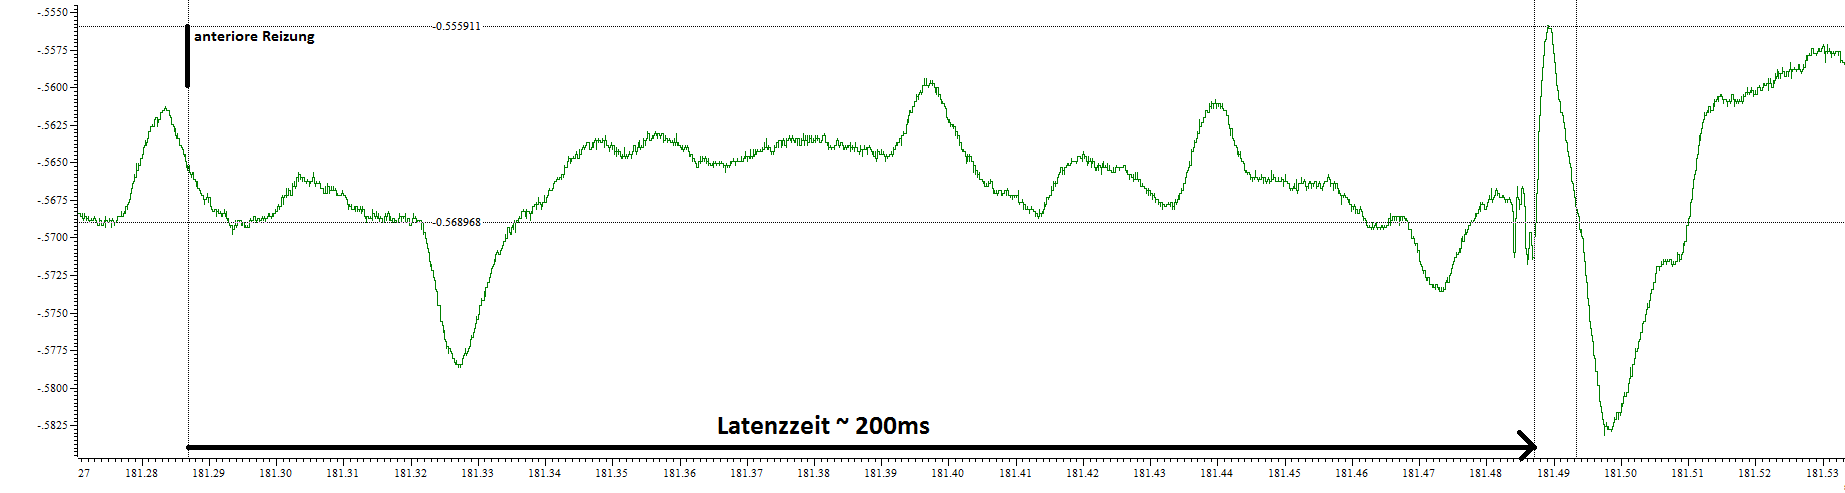
\includegraphics[width=\textwidth]{images/Exp2_aR.png}
    \caption{Myogramm für anteriore Reizung}
\end{figure}
\begin{figure}[H]
    \centering
        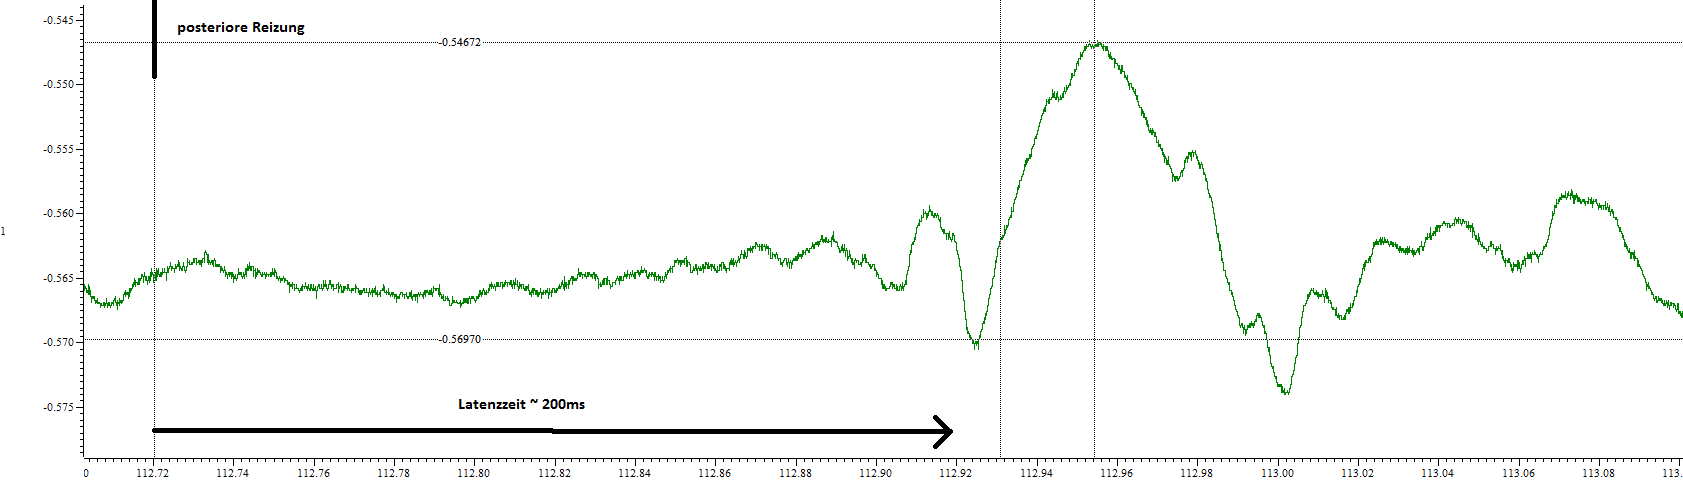
\includegraphics[width=\textwidth]{images/Exp2_pR.png}
    \caption{Myogramm für posteriore Reizung}
\end{figure}

\subsection{Reizschwellenmessung und Fortleitungsgeschwindigkeit}
Der Schwellwert für die Erzeugung \textbf{eines} Aktionspotentials lag bei 3,5 V.\\
Durchschnittliche Werte für ein Aktionspotential beim Schwellwert 3,5 V:\\
Amplitude: 4,04 mV (sd: 0,08)\\
Dauer: 1,75 ms (sd: 0,25)\\
Latenzzeit: 12,5 ms (sd: 0,5)\\ \\
Der Schwellwert für die Erzeugung von \textbf{zwei} Aktionspotentialen lag bei 5 V.\\
Durchschnittliche Werte für das erste Aktionspotential beim Schwellwert 5 V:\\
Amplitude: 27,49 mV (sd: 2,28)\\
Dauer: 0,433 ms (sd: 0,058)\\
Latenzzeit: 4 ms (sd: 0,0)\\ \\
Durchschnittliche Werte für das zweite Aktionspotential beim Schwellwert 5 V:\\
Amplitude: 18,2 mV (sd: 7,45)\\
Dauer: 0,767 ms (sd: 0,058)\\
Latenzzeit: 6 ms (sd: 0,0)\\
\begin{figure}[H]
    \centering
        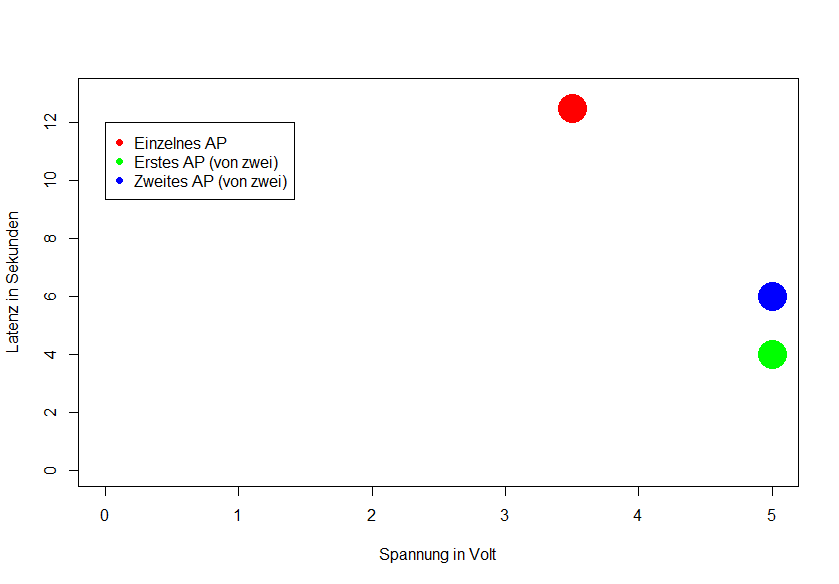
\includegraphics[width=\textwidth]{images/Vergleich_Spannung_Latenz.png}
    \caption{Vergleich Schwellspannung zu Latenzzeit. Bei Reizung mit höherer Spannung wird schneller ein Aktionspotential ausgelöst.}
\end{figure}
Es konnten nur Aktionspotentiale des lateralen Riesenfasersystems (LRF) beobachtet werden. Zu beobachten war auch, dass bei der mechanischen Reizung auftretende LRF Aktionspotentiale größere Amplitude und Dauer hatten, allerdings auch eine deutlich höhere Latenzzeit.\\ \\
Die Geschwindigkeit der Reizweiterleitung für LRF ist vom Abstand der Reiz- zu den Messelektroden abhängig, den wir uns allerdings nicht notiert hatten. Ausgehend von einem beispielhaften Abstand von 10cm ergibt sich eine Geschwindigkeit von 8 m/s bei einem Reiz von 3,5 V und eine Geschwindigkeit von 25 m/s bei einem Reiz von 5V.

\subsection{Refraktärphase bei elektrischer Reizung}
Wir haben unserer Messungen bei 5 Volt und einem Delay von 20 ms begonnen und konnten ab einem zeitlichen Abstand von 10 ms der Impulse kein zweites Aktionspotential mehr beobachten. Allerdings ist uns bei dem Auswerten der Daten aufgefallen, dass unsere Messungen leider unbrauchbar sind, da wir im Nachhinein keinen Twin Pulse mehr finden konnten, bei dem nur ein Aktionpotential ausgelöst wurde. Desweiteren hätten wir die Spannungsstärke anfänglich nicht auf 5 Volt stellen dürfen, weil dieses unsere Schwelle zur Auslösung von zwei Aktionspotentialen aus Experiment 3.4 war. Die zu erwartenden Ergebnisse und Hintergrundinformationen zum Experiment finden sich in Kapitel 4.3.

\section{Diskussion}

\subsection{Mechanische Reizung}
Die geringere Latenzzeit bei posteriorer Reizung liegt daran, dass die Messelektroden näher am posterioren Ende des Wurms lagen. Dies dürfte auch der Grund sein, warum die gemessene Amplitude bei posteriorer Reizung größer ist.

\subsection{Reizschwellmessung und Fortleitungsgeschwindigkeit}
Bei der Reizung mit 5V konnten zwei Aktionspotentiale pro Reizung beobachtet werden. Bei diesem Schwellwert liegt nach der absoluten Refraktärphase noch ausreichend Spannung an, um ein weiteres Aktionspotential auszulösen. Da dies in der relativen Refraktärphase geschieht, ist die Amplitude des zweiten AP kleiner, und die Dauer ist etwas länger als beim ersten AP.

\subsection{Refraktärphase bei elektrischer Reizung}
Ziel war es die Refraktärzeit (den Zeitraum nach Auslösung eines Aktionspotentials, in dem die auslösende Nervenzelle temporär nicht erneut auf einen Reiz reagieren kann) zu bestimmen. Nach der Auslösung eines Aktionspotentials schließen sich die betroffenen Natrium Kanäle selbständig und sind dann nicht sofort wieder bereit, sich zu öffnen. Bei der im Experiment gesuchten \textit{absoluten} Refraktärzeit handelt es sich um die Zeit bei der kein Aktionspotential ausgelöst werden, unabhängig von dessen Reizstärke. Laut unseren Nachforschungen würde die erwartete absolute Refraktärzeit bei etwa 2ms liegen.

\printbibliography

\end{document}